\problemname{Mountain Range}
Markus often gets bored during math class, and has therefore started drawing different landscapes in his notebook. He has for example discovered the following procedure for easily drawing a nice mountain range:

\begin{enumerate}
\item Start by drawing the ground as a horizontal line.
\item Then pick a number of points above the ground. These points will represent mountain peaks.
\item From each point, draw two lines that intersect the ground at a 45 degree angle, creating a number of isosceles right triangles.
\item Then fill in the triangles. Note that the triangles may overlap, and in that case you do not need to fill all of them in completely.
\end{enumerate}

\noindent Given $N$ points drawn above the ground, compute the area that needs to be filled in to create the mountain range.

\section*{Input}
The first line contains the number $N$. The following $N$ lines each contain two integers $X$ and $Y$, separated by spaces. These describe the coordinates of the points that were drawn.

\section*{Output}
Your program should output a single number on a line, the total area that needs to be filled in.

\section*{Explanation of Samples}

\begin{figure}[ht!]
\centering
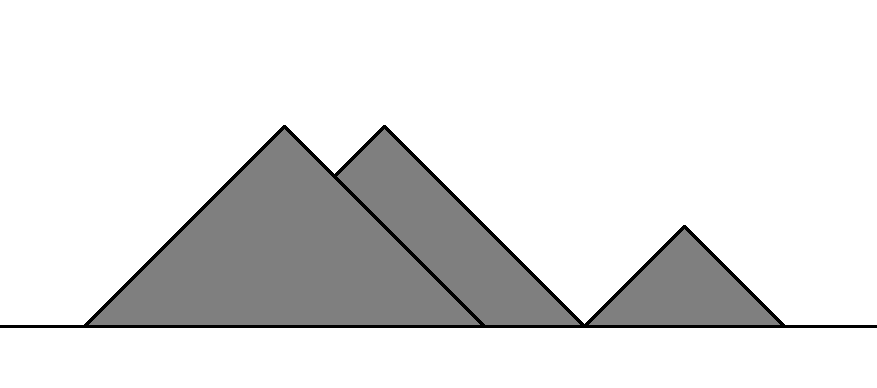
\includegraphics[width=0.7\textwidth]{bergskedja.png}
\caption{An illustration of the first example.}
\label{overflow}
\end{figure}

% TODO: beskriv med text?

\section*{Scoring}
Your solution will be tested on a set of test groups. To earn points for a group,
you must pass all test cases in that group.

\begin{tabular}{| l | l | l | l |}
\hline
Group & Points & Constraints \\ \hline
1     & 20         &  $1 \le N \le 100, -100 \le X \le 100, 0 \le Y \le 100$ \\ \hline
2     & 20         &  $1 \le N \le 100\,000, -1\,000 \le X \le 1\,000, 0 \le Y \le 1\,000$ \\ \hline
3     & 60         &  $1 \le N\le 100\,000, -100\,000 \le X \le 100\,000, 0 \le Y \le 10\,000$\\ \hline
\end{tabular}

\section*{Precision}
An answer to this problem will be considered correct if the absolute error is less than $10^{-3}$. Note that for full points one needs to be able to output answers with many digits of precision (see sample 3). If you are using C++ and cout, for example, you will need to specify the desired precision before outputting the answer.
